\documentclass[a4paper,12pt]{article}
   % Packages and definitions:
   % {
      \usepackage{float}
      \usepackage[english]{babel}
      \usepackage[utf8]{inputenc}
      \usepackage{amsmath}
      \usepackage{amssymb}
      \usepackage{color}
      \usepackage{subcaption}
      \usepackage{booktabs}
      \usepackage{tikz}
      \usepackage{multirow}
      \usetikzlibrary{decorations.pathreplacing}
      \usepackage{graphicx,epstopdf}
      \usepackage{cleveref}
      \usepackage{collcell} % loads array
      \usepackage{listings}
      \usepackage{algorithm}
      \usepackage{algpseudocode}
      \usepackage{epstopdf}
      \newcolumntype{m}{>{$} r <{$}}
      \newcolumntype{u}{>{$[\collectcell\si} l <{\endcollectcell]$}}
      \newcommand{\approxtext}[1]{\ensuremath{\stackrel{\text{#1}}{=}}}
      \newcommand{\matr}[1]{\mathbf{#1}}
      \newcommand{\partt}[2]{\ensuremath{\dfrac{\d {#1}}{\partial {#2}}}}
      \renewcommand{\d}[1]{\ensuremath{\operatorname{d}\!{#1}}} % non-italized differentials
      \newcommand{\h}[0]{\ensuremath{\hbar}} % hbar
      \newcommand{\qed}[0]{\ensuremath{\tag*{$\square$}}} % QED square
      \def\changemargin#1#2{\list{}{\rightmargin#2\leftmargin#1}\item[]}
      \let\endchangemargin=\endlist 
      \usepackage{amsthm}
      \theoremstyle{plain}
      \newtheorem{thm}{theorem} % reset theorem numbering for each chapter
      \theoremstyle{definition}
      \newtheorem{defn}[thm]{definition} % definition numbers are dependent on theorem numbers
      \newtheorem{exmp}[thm]{example} % same for example numbers
      \bibliographystyle{natbib}
      \renewcommand{\theequation}{\thesection.\arabic{equation}}
      \newcommand{\ts}{\textsuperscript} 

      \definecolor{dkgreen}{rgb}{0,0.6,0}
      \definecolor{gray}{rgb}{0.5,0.5,0.5}
      \definecolor{mauve}{rgb}{0.58,0,0.82}

      \lstset{frame=tb,
        language=Java,
        aboveskip=3mm,
        belowskip=3mm,
        showstringspaces=false,
        columns=flexible,
        basicstyle={\small\ttfamily},
        numbers=none,
        numberstyle=\tiny\color{gray},
        keywordstyle=\color{blue},
        commentstyle=\color{dkgreen},
        stringstyle=\color{mauve},
        breaklines=true,
        breakatwhitespace=true,
        tabsize=3
      }
% }
\title
{
	\textbf
	{
      Single and Multi-layer perceptrons for classifications and predictions of
      time series
   }
}

\author{Henrik Åhl\\}
\date{\today}

\begin{document}
\begin{titlepage}
	
   \maketitle 
	\begin{center}
		\phantom{a}
		{Department of Astronomy and Theoretical Physics, Lund University}
		\\[2cm]
		{Project supervised by Mattias Ohlsson}
		\vfill
		\includegraphics[height=4cm]{logocLUeng.pdf}
	\end{center}
	\thispagestyle{empty} % do not count pages just yet

\end{titlepage}

\vspace{5cm}
\noindent\textit{If you can't go with the scientific argument -- \\go with the
non-scientific~argument.}\\ --- Mattias Ohlsson, 2015
\newpage

\section{Introduction}
   Neural networks can be used for a wide range of purposes, ranging from
   function approximation to identifying patterns in images. Although the
   networks themselves can be constructed to be however complicated the creator
   wishes, relatively simple networks can be shown to be able to solve
   complicated tasks. Especially single-layer perceptrons, as are the main study in
   this report, are able to perform surprisingly complex tasks.

\section{Problems}
	\setcounter{equation}{0}
   \subsection{XOR logic}
      In the XOR problematic, it is easy to realize that the problem cannot be
      solved by a perceptron without hidden nodes; the reason being best
      visualised graphically, where it can be seen that the decision boundary
      for the network is constructed by a single linear function in the
      $x_1$--$x_2$ plane. Since the desired outputs are not separable by a linear
      function, it is impossible for the network to solve the problem. 

      Using simple gradient descent learing, i.e. without adaptive learning
      rates and momentum included, the network is contrary to the intuitive idea
      not able to learn to circumvent the problematic. Out of 1000 simulated networks, not a
      single one produces a solution to the problem. When instead
      introducting different mechanics to the learning algorithm, the results
      found in \cref{tab:xor} display the performances measured on different
      version of the Gradient Descent (GD) method, as well as the
      Levenberg-Marquardt (LM) method. 

      \begin{table}[H]
         \centering
         \begin{tabular}{lr}
            \toprule
            \textbf{Method} & \textbf{Success rate [\%]}\\ 
            \midrule
            GD & 0.0 \\
            GD + momentum & 0.0 \\
            GD + adaptive learning rate & 25.3 \\
            GD + both & 29.1 \\
            LM & 49.1 \\ \bottomrule
         \end{tabular}
         \caption{Results when trying to solve the XOR logic with a neural net
         constructed by two hidden nodes. Every method experienced 1000
      simulations.}
         \label{tab:xor}
      \end{table}

      When instead increasing the number of nodes, all methods but the ordinary
      GD algorithm, as well as the GD with a momentum modification, produce results 
      rapidly converging towards 100 \% correct
      classifications. Already at 4 hidden nodes, all but the original GD and
      the momentum method
      give results with $>$$95$ \% correct classifications over 1000 simulations.
      The ordinary GD method instead only produces the correct result 2 \% of the
      time with as many as 50 hidden nodes. Similar results apply for the
      momentum version of the algorithm. 
      
  \subsection{Synthetic Data} 
      Using the second given synthetic data set, a graphical visualization of the data, as
      can be seen in \cref{fig:6} helps understand why the problem is solvable
      by a network with a single node; clearly the two classes are clustered in
      such a way that a linear boundary is sufficient to discern the class of
      the data in an adequate way. Plotting the full data set (not here
      depicted) further shows the nature of this specific feature of the data. 

      \begin{figure}[H]
         \centering
         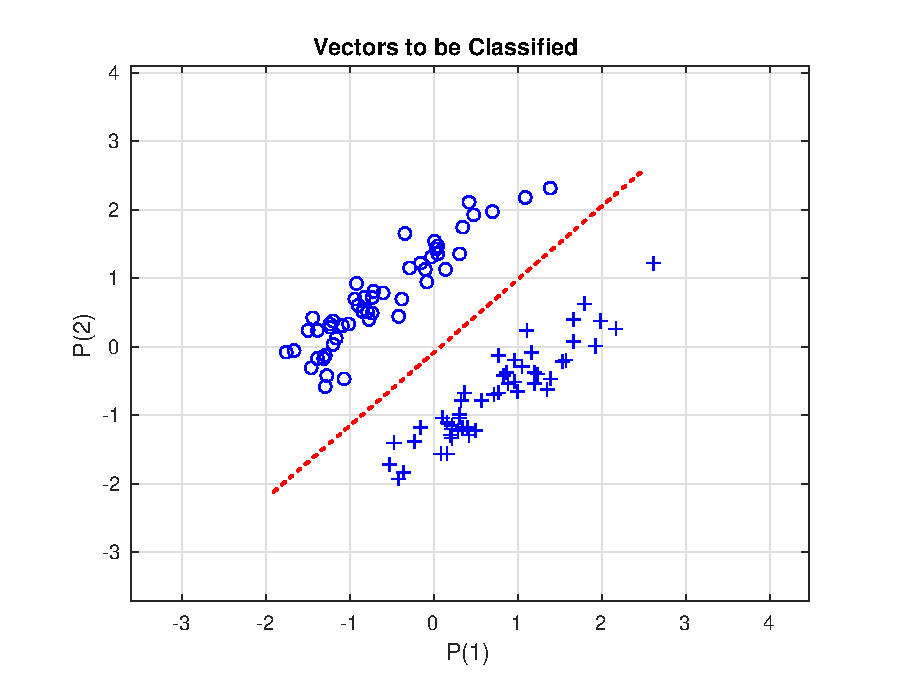
\includegraphics[scale=.6]{6}
         \label{fig:6}
         \caption{Graphical results of the training performance for the synthetic
         data set. The linear function shows the decision boundary produced by the
         neural network.}
      \end{figure}

      Also when performing the analogue analysis on the first data set, a visual
      representation is beneficial in understanding the problematic. In
      \cref{fig:8_data} the validation output of a 15 node network can be seen, which
      highlights the significant overlap between the two classes.
      
      \begin{figure}[H]
         \centering
         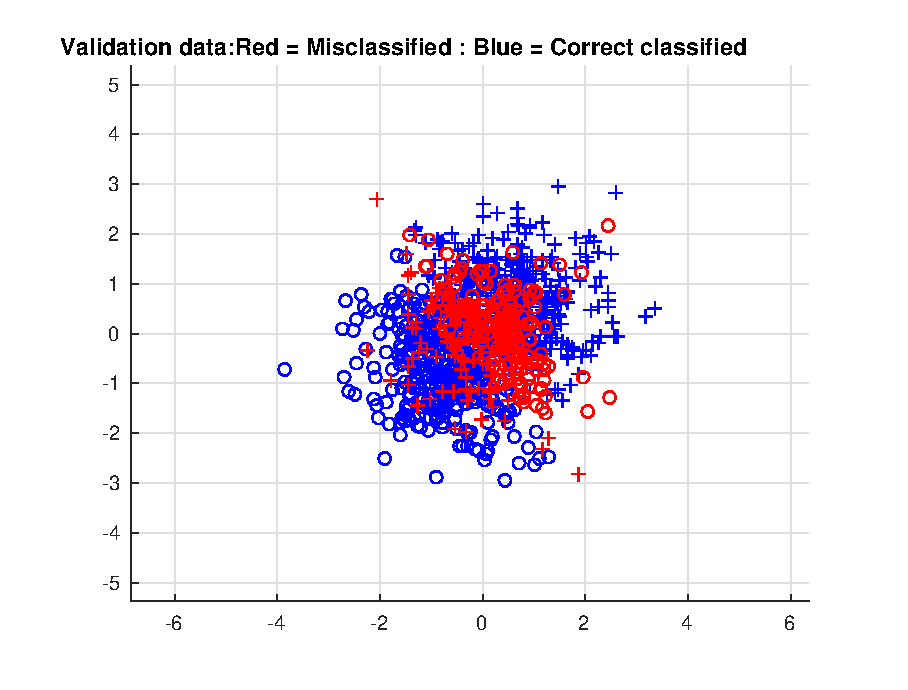
\includegraphics[scale=.6]{8_data}
         \label{fig:8_data}
         \caption{Depiction of the problematic in trying to discern the two
         classes from each other. The graph itself shows the validation performance of a
         15 node network.}
      \end{figure}

      In examining the occurence of overtraining, as can be investigated in comparison between
      fig.~3 and fig.~4, it can somewhat unintuitively
      be seen that although it might be so that the network indeed adapts to
      individual data points more and more as additional nodes are added to the
      network, it does not seem to be biased so heavily that the approximation
      turns downright bad. Indeed, single data points can be noted to have
      greater weight with more nodes, although since the number of weights are
      increased so much between the two graphs, it would seem natural if more
      overtraining were present.  

      \begin{figure}[H]
         \vspace*{1cm}
         \hspace*{-2cm}
         \centering
         \begin{minipage}[t]{.6\textwidth}		
            \vspace{0pt}
            \centering
            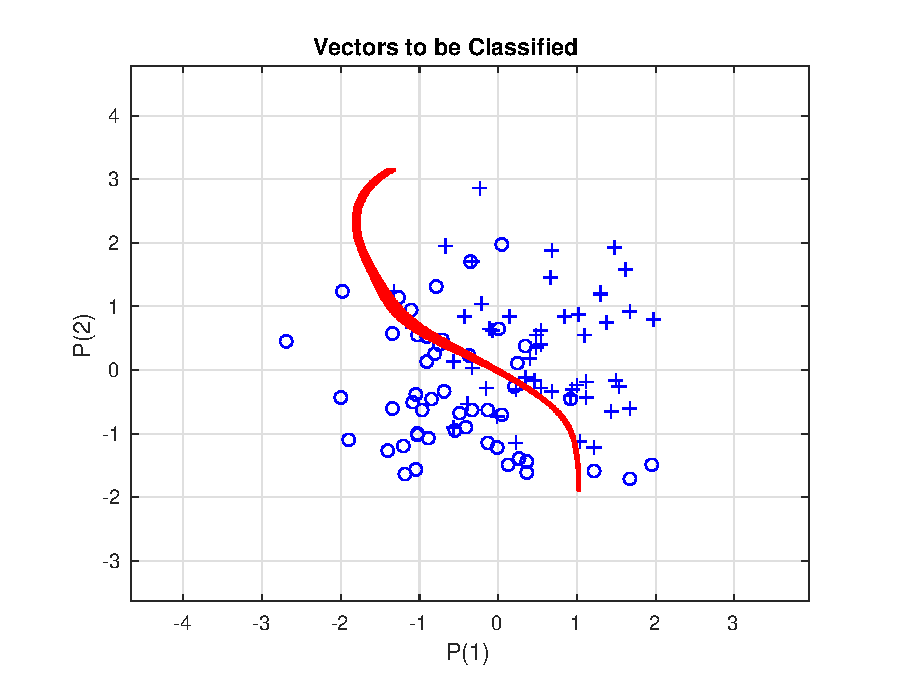
\includegraphics[scale=.6]{8_12_nodes}
            \label{fig:8_12_nodes}
            \caption{Classification output for synthetic data set 1, with 12
            hidden nodes.}
         \end{minipage}~\hspace*{1em}
         \begin{minipage}[t]{.6\textwidth}		
            \vspace{0pt}
            \centering
            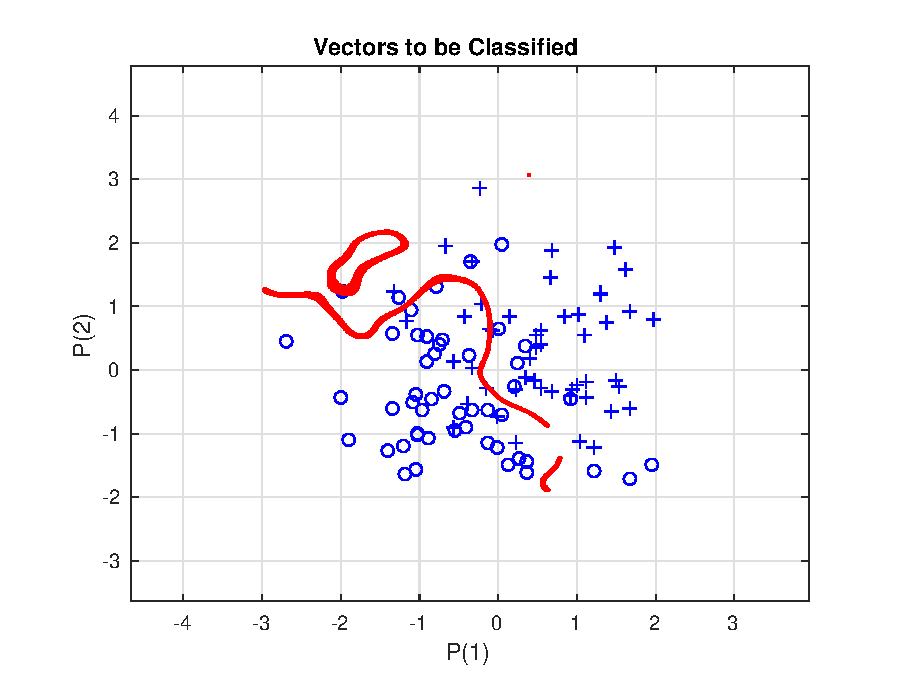
\includegraphics[scale=.6]{8_100_nodes}
            \label{fig:8_100_nodes}
            \caption{Classification output for synthetic data set 1, with 100
            hidden nodes. Note that there are vague signs of overtraining relative to
            fig.~3.}
         \end{minipage}
      \end{figure}
      
      \begin{figure}[H]
         \centering
         \resizebox{.7\textwidth}{!}{% GNUPLOT: LaTeX picture with Postscript
\begingroup
  \makeatletter
  \providecommand\color[2][]{%
    \GenericError{(gnuplot) \space\space\space\@spaces}{%
      Package color not loaded in conjunction with
      terminal option `colourtext'%
    }{See the gnuplot documentation for explanation.%
    }{Either use 'blacktext' in gnuplot or load the package
      color.sty in LaTeX.}%
    \renewcommand\color[2][]{}%
  }%
  \providecommand\includegraphics[2][]{%
    \GenericError{(gnuplot) \space\space\space\@spaces}{%
      Package graphicx or graphics not loaded%
    }{See the gnuplot documentation for explanation.%
    }{The gnuplot epslatex terminal needs graphicx.sty or graphics.sty.}%
    \renewcommand\includegraphics[2][]{}%
  }%
  \providecommand\rotatebox[2]{#2}%
  \@ifundefined{ifGPcolor}{%
    \newif\ifGPcolor
    \GPcolorfalse
  }{}%
  \@ifundefined{ifGPblacktext}{%
    \newif\ifGPblacktext
    \GPblacktexttrue
  }{}%
  % define a \g@addto@macro without @ in the name:
  \let\gplgaddtomacro\g@addto@macro
  % define empty templates for all commands taking text:
  \gdef\gplbacktext{}%
  \gdef\gplfronttext{}%
  \makeatother
  \ifGPblacktext
    % no textcolor at all
    \def\colorrgb#1{}%
    \def\colorgray#1{}%
  \else
    % gray or color?
    \ifGPcolor
      \def\colorrgb#1{\color[rgb]{#1}}%
      \def\colorgray#1{\color[gray]{#1}}%
      \expandafter\def\csname LTw\endcsname{\color{white}}%
      \expandafter\def\csname LTb\endcsname{\color{black}}%
      \expandafter\def\csname LTa\endcsname{\color{black}}%
      \expandafter\def\csname LT0\endcsname{\color[rgb]{1,0,0}}%
      \expandafter\def\csname LT1\endcsname{\color[rgb]{0,1,0}}%
      \expandafter\def\csname LT2\endcsname{\color[rgb]{0,0,1}}%
      \expandafter\def\csname LT3\endcsname{\color[rgb]{1,0,1}}%
      \expandafter\def\csname LT4\endcsname{\color[rgb]{0,1,1}}%
      \expandafter\def\csname LT5\endcsname{\color[rgb]{1,1,0}}%
      \expandafter\def\csname LT6\endcsname{\color[rgb]{0,0,0}}%
      \expandafter\def\csname LT7\endcsname{\color[rgb]{1,0.3,0}}%
      \expandafter\def\csname LT8\endcsname{\color[rgb]{0.5,0.5,0.5}}%
    \else
      % gray
      \def\colorrgb#1{\color{black}}%
      \def\colorgray#1{\color[gray]{#1}}%
      \expandafter\def\csname LTw\endcsname{\color{white}}%
      \expandafter\def\csname LTb\endcsname{\color{black}}%
      \expandafter\def\csname LTa\endcsname{\color{black}}%
      \expandafter\def\csname LT0\endcsname{\color{black}}%
      \expandafter\def\csname LT1\endcsname{\color{black}}%
      \expandafter\def\csname LT2\endcsname{\color{black}}%
      \expandafter\def\csname LT3\endcsname{\color{black}}%
      \expandafter\def\csname LT4\endcsname{\color{black}}%
      \expandafter\def\csname LT5\endcsname{\color{black}}%
      \expandafter\def\csname LT6\endcsname{\color{black}}%
      \expandafter\def\csname LT7\endcsname{\color{black}}%
      \expandafter\def\csname LT8\endcsname{\color{black}}%
    \fi
  \fi
  \setlength{\unitlength}{0.0500bp}%
  \begin{picture}(7200.00,5040.00)%
    \gplgaddtomacro\gplbacktext{%
      \colorrgb{0.42,0.42,0.42}%
      \put(814,704){\makebox(0,0)[r]{\strut{} 72}}%
      \colorrgb{0.42,0.42,0.42}%
      \put(814,1383){\makebox(0,0)[r]{\strut{} 74}}%
      \colorrgb{0.42,0.42,0.42}%
      \put(814,2061){\makebox(0,0)[r]{\strut{} 76}}%
      \colorrgb{0.42,0.42,0.42}%
      \put(814,2740){\makebox(0,0)[r]{\strut{} 78}}%
      \colorrgb{0.42,0.42,0.42}%
      \put(814,3418){\makebox(0,0)[r]{\strut{} 80}}%
      \colorrgb{0.42,0.42,0.42}%
      \put(814,4097){\makebox(0,0)[r]{\strut{} 82}}%
      \colorrgb{0.42,0.42,0.42}%
      \put(814,4775){\makebox(0,0)[r]{\strut{} 84}}%
      \colorrgb{0.42,0.42,0.42}%
      \put(946,484){\makebox(0,0){\strut{} 2}}%
      \colorrgb{0.42,0.42,0.42}%
      \put(1783,484){\makebox(0,0){\strut{} 4}}%
      \colorrgb{0.42,0.42,0.42}%
      \put(2619,484){\makebox(0,0){\strut{} 6}}%
      \colorrgb{0.42,0.42,0.42}%
      \put(3456,484){\makebox(0,0){\strut{} 8}}%
      \colorrgb{0.42,0.42,0.42}%
      \put(4293,484){\makebox(0,0){\strut{} 10}}%
      \colorrgb{0.42,0.42,0.42}%
      \put(5130,484){\makebox(0,0){\strut{} 12}}%
      \colorrgb{0.42,0.42,0.42}%
      \put(5966,484){\makebox(0,0){\strut{} 14}}%
      \colorrgb{0.42,0.42,0.42}%
      \put(6803,484){\makebox(0,0){\strut{} 16}}%
      \colorrgb{0.42,0.42,0.42}%
      \put(176,2739){\rotatebox{-270}{\makebox(0,0){\strut{}Performance [\%]}}}%
      \colorrgb{0.42,0.42,0.42}%
      \put(3874,154){\makebox(0,0){\strut{}Nodes}}%
      \colorrgb{0.42,0.42,0.42}%
      \put(3874,4665){\makebox(0,0){\strut{}}}%
    }%
    \gplgaddtomacro\gplfronttext{%
      \csname LTb\endcsname%
      \put(5804,4602){\makebox(0,0)[r]{\strut{}Training}}%
      \csname LTb\endcsname%
      \put(5804,4382){\makebox(0,0)[r]{\strut{}Validation}}%
    }%
    \gplbacktext
    \put(0,0){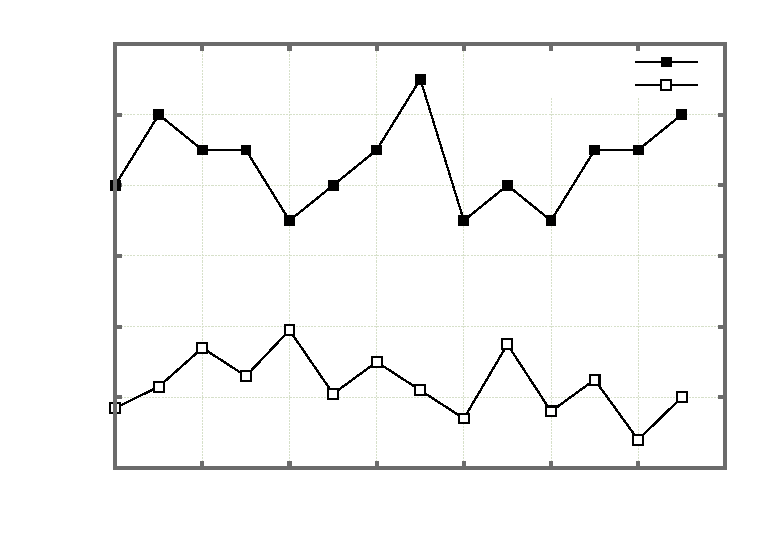
\includegraphics{7}}%
    \gplfronttext
  \end{picture}%
\endgroup
}
         \caption{Training versus validation performance (fraction of correct
         classifications) on synthetic data set 1. Note that the validation
         performance is consistently lower than the training one.}
         \label{fig:7_and_8_comp}            
      \end{figure}
      
      Increasing the number of nodes used seems not to affect the overall
      performance in any determinable way, as \cref{fig:7_and_8_comp} signifies.
      Instead, the performance fluctuates stadily around the same output as the
      linear MLP manages to produce.

      For the final synthetic data set, one can at observing the data set
      itself realize that it ought to require at least three hidden nodes in order
      to classify the network properly. This is because of the enclosedness that
      forelie, where one class is wholly enclosed by the other in the data
      plane; since it would require three straight lines in order to enclose
      an area in a plane, it would seem natural that at least three nodes are
      required. The conclusion is solely based on the fact that a node in a
      network principally represents a linear delimiter in the input space.
      
      \begin{figure}[H]
         \centering
         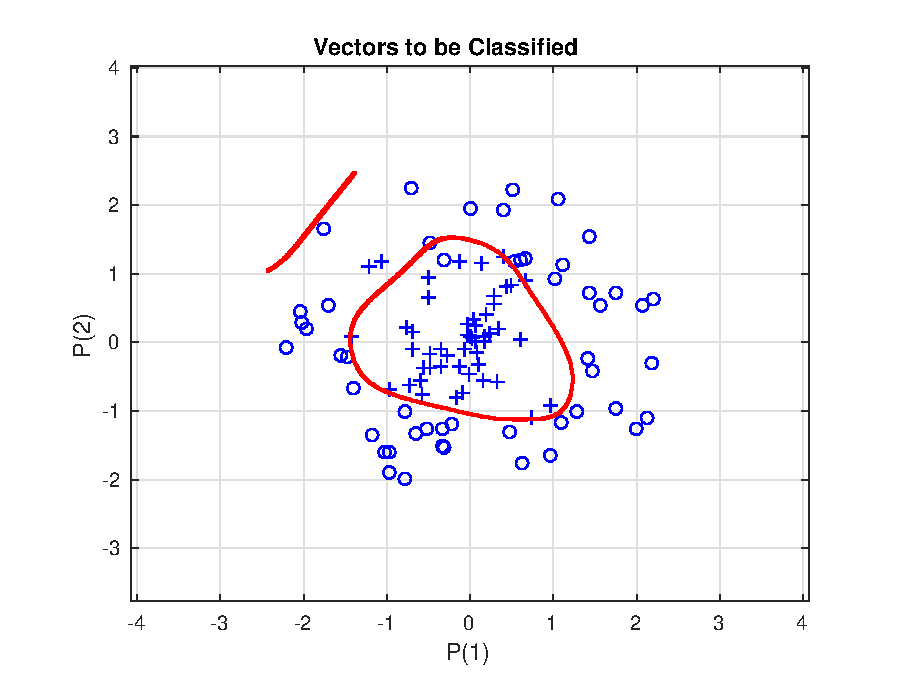
\includegraphics[scale=.6]{9_15_nodes}
         \label{fig:9_data}
         \caption{Training sample of synthetic data set 3. Graph shows training classification for a 15 node
      network.}
      \end{figure}
      
      \begin{figure}[H]
         \centering
         \resizebox{.7\textwidth}{!}{% GNUPLOT: LaTeX picture with Postscript
\begingroup
  \makeatletter
  \providecommand\color[2][]{%
    \GenericError{(gnuplot) \space\space\space\@spaces}{%
      Package color not loaded in conjunction with
      terminal option `colourtext'%
    }{See the gnuplot documentation for explanation.%
    }{Either use 'blacktext' in gnuplot or load the package
      color.sty in LaTeX.}%
    \renewcommand\color[2][]{}%
  }%
  \providecommand\includegraphics[2][]{%
    \GenericError{(gnuplot) \space\space\space\@spaces}{%
      Package graphicx or graphics not loaded%
    }{See the gnuplot documentation for explanation.%
    }{The gnuplot epslatex terminal needs graphicx.sty or graphics.sty.}%
    \renewcommand\includegraphics[2][]{}%
  }%
  \providecommand\rotatebox[2]{#2}%
  \@ifundefined{ifGPcolor}{%
    \newif\ifGPcolor
    \GPcolorfalse
  }{}%
  \@ifundefined{ifGPblacktext}{%
    \newif\ifGPblacktext
    \GPblacktexttrue
  }{}%
  % define a \g@addto@macro without @ in the name:
  \let\gplgaddtomacro\g@addto@macro
  % define empty templates for all commands taking text:
  \gdef\gplbacktext{}%
  \gdef\gplfronttext{}%
  \makeatother
  \ifGPblacktext
    % no textcolor at all
    \def\colorrgb#1{}%
    \def\colorgray#1{}%
  \else
    % gray or color?
    \ifGPcolor
      \def\colorrgb#1{\color[rgb]{#1}}%
      \def\colorgray#1{\color[gray]{#1}}%
      \expandafter\def\csname LTw\endcsname{\color{white}}%
      \expandafter\def\csname LTb\endcsname{\color{black}}%
      \expandafter\def\csname LTa\endcsname{\color{black}}%
      \expandafter\def\csname LT0\endcsname{\color[rgb]{1,0,0}}%
      \expandafter\def\csname LT1\endcsname{\color[rgb]{0,1,0}}%
      \expandafter\def\csname LT2\endcsname{\color[rgb]{0,0,1}}%
      \expandafter\def\csname LT3\endcsname{\color[rgb]{1,0,1}}%
      \expandafter\def\csname LT4\endcsname{\color[rgb]{0,1,1}}%
      \expandafter\def\csname LT5\endcsname{\color[rgb]{1,1,0}}%
      \expandafter\def\csname LT6\endcsname{\color[rgb]{0,0,0}}%
      \expandafter\def\csname LT7\endcsname{\color[rgb]{1,0.3,0}}%
      \expandafter\def\csname LT8\endcsname{\color[rgb]{0.5,0.5,0.5}}%
    \else
      % gray
      \def\colorrgb#1{\color{black}}%
      \def\colorgray#1{\color[gray]{#1}}%
      \expandafter\def\csname LTw\endcsname{\color{white}}%
      \expandafter\def\csname LTb\endcsname{\color{black}}%
      \expandafter\def\csname LTa\endcsname{\color{black}}%
      \expandafter\def\csname LT0\endcsname{\color{black}}%
      \expandafter\def\csname LT1\endcsname{\color{black}}%
      \expandafter\def\csname LT2\endcsname{\color{black}}%
      \expandafter\def\csname LT3\endcsname{\color{black}}%
      \expandafter\def\csname LT4\endcsname{\color{black}}%
      \expandafter\def\csname LT5\endcsname{\color{black}}%
      \expandafter\def\csname LT6\endcsname{\color{black}}%
      \expandafter\def\csname LT7\endcsname{\color{black}}%
      \expandafter\def\csname LT8\endcsname{\color{black}}%
    \fi
  \fi
  \setlength{\unitlength}{0.0500bp}%
  \begin{picture}(7200.00,5040.00)%
    \gplgaddtomacro\gplbacktext{%
      \colorrgb{0.42,0.42,0.42}%
      \put(814,704){\makebox(0,0)[r]{\strut{} 60}}%
      \colorrgb{0.42,0.42,0.42}%
      \put(814,1286){\makebox(0,0)[r]{\strut{} 65}}%
      \colorrgb{0.42,0.42,0.42}%
      \put(814,1867){\makebox(0,0)[r]{\strut{} 70}}%
      \colorrgb{0.42,0.42,0.42}%
      \put(814,2449){\makebox(0,0)[r]{\strut{} 75}}%
      \colorrgb{0.42,0.42,0.42}%
      \put(814,3030){\makebox(0,0)[r]{\strut{} 80}}%
      \colorrgb{0.42,0.42,0.42}%
      \put(814,3612){\makebox(0,0)[r]{\strut{} 85}}%
      \colorrgb{0.42,0.42,0.42}%
      \put(814,4193){\makebox(0,0)[r]{\strut{} 90}}%
      \colorrgb{0.42,0.42,0.42}%
      \put(814,4775){\makebox(0,0)[r]{\strut{} 95}}%
      \colorrgb{0.42,0.42,0.42}%
      \put(946,484){\makebox(0,0){\strut{} 0}}%
      \colorrgb{0.42,0.42,0.42}%
      \put(1678,484){\makebox(0,0){\strut{} 2}}%
      \colorrgb{0.42,0.42,0.42}%
      \put(2410,484){\makebox(0,0){\strut{} 4}}%
      \colorrgb{0.42,0.42,0.42}%
      \put(3142,484){\makebox(0,0){\strut{} 6}}%
      \colorrgb{0.42,0.42,0.42}%
      \put(3875,484){\makebox(0,0){\strut{} 8}}%
      \colorrgb{0.42,0.42,0.42}%
      \put(4607,484){\makebox(0,0){\strut{} 10}}%
      \colorrgb{0.42,0.42,0.42}%
      \put(5339,484){\makebox(0,0){\strut{} 12}}%
      \colorrgb{0.42,0.42,0.42}%
      \put(6071,484){\makebox(0,0){\strut{} 14}}%
      \colorrgb{0.42,0.42,0.42}%
      \put(6803,484){\makebox(0,0){\strut{} 16}}%
      \colorrgb{0.42,0.42,0.42}%
      \put(176,2739){\rotatebox{-270}{\makebox(0,0){\strut{}Performance [\%]}}}%
      \colorrgb{0.42,0.42,0.42}%
      \put(3874,154){\makebox(0,0){\strut{}Nodes}}%
      \colorrgb{0.42,0.42,0.42}%
      \put(3874,4665){\makebox(0,0){\strut{}}}%
    }%
    \gplgaddtomacro\gplfronttext{%
      \csname LTb\endcsname%
      \put(5804,4602){\makebox(0,0)[r]{\strut{}Validation}}%
    }%
    \gplbacktext
    \put(0,0){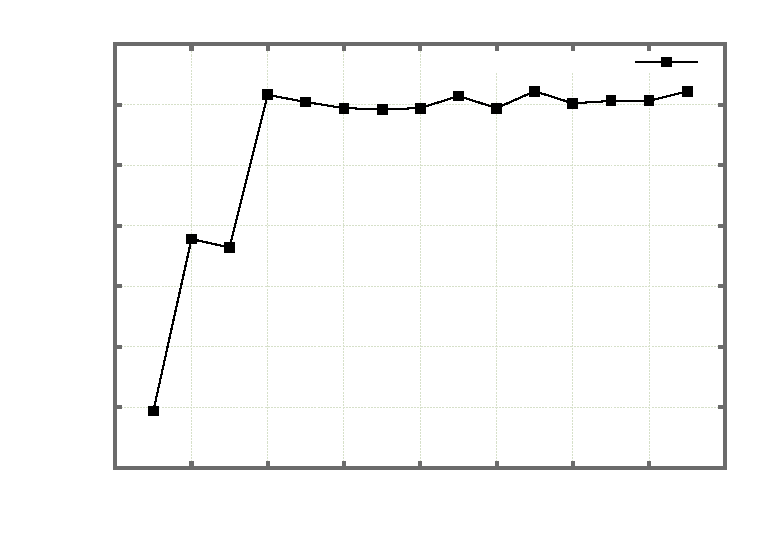
\includegraphics{9}}%
    \gplfronttext
  \end{picture}%
\endgroup
}
         \caption{Validation performance for different sizes of a single-layer
         MLP on synthetic data set 3.}
         \label{fig:9}            
      \end{figure}
   
      It can be noted from the validation performance chart in \cref{fig:9} that
      as long as at least 4 nodes are present, the network is able to correctly
      classify the data to a large extent. It can principally be assumed that there would be
      an increase in performance the more nodes are added to the network (over a
      sample of simulations), although some error is bound to be present due to
      the slight overlap between the data sets. It ought to be probable that the
      convergence value inherent to the problem is close to the plateau visible
      in the performance graph however. 

   \subsection{Liver Data}
      For the liver data set, all different methods available for the exercise
      were tested, simulated with nodes ranging from one to 15. As the data was
      assumed to be supposed to classify healthy/non-healty individuals, the
      specificity, i.e. the measure corresponding to the ability to find as many
      (again: assumed) non-healhty individuals, was chosen. Of all the methods,
      the Scaled Conjugate Gradient method with a single layer and 11 nodes was
      the must successful in this regards, being able to find 45.45 \% of the
      data belonging to class 0 (non-healthy). This should however be put in relation to the
      sensitivity, which assumed a value of 84.06 \%. In other words, the network
      did not wrongly classify all too many ``healthy'' individuals. It must 
      nontheless be stressed that the variance for all the methods was
      high in relation to the performance, so that further results would be
      needed to draw realistical conclusions about the preferable algorithm.

   \subsection{Time Series}
      \begin{figure}[H]
         \centering
         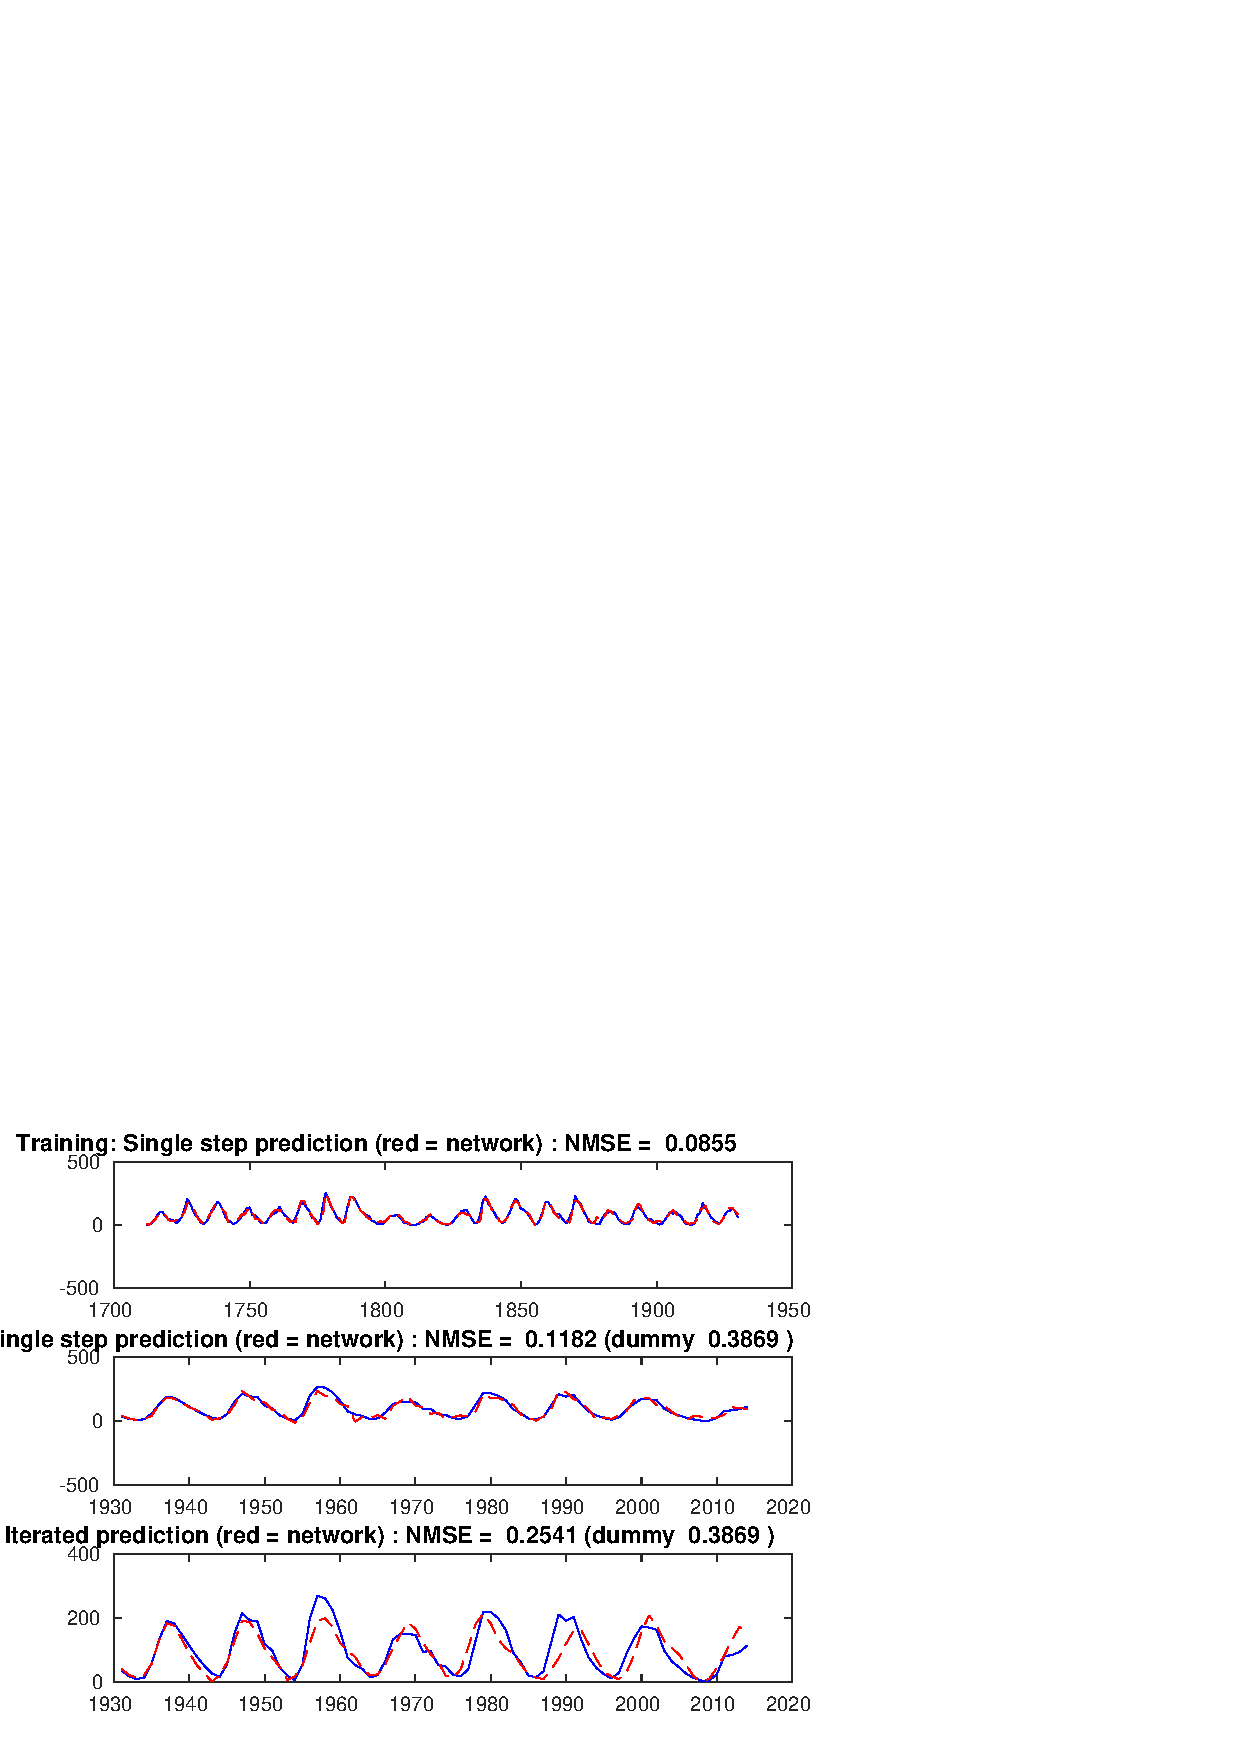
\includegraphics[scale=.8]{11_7_nodes_levenberg}
         \caption{Performance for single-layer network with 7 hidden nodes and
         the LM algorithm on the sunspot data.}
         \label{fig:11}
      \end{figure}
      
      In finding an underlying pattern for the sunspots, who seem to exhibit an
      oscillating behaviour, peaking roughly every eleven years, all methods
      were again tested on the data set. The most efficient proved to be the
      Levenberg method, which managed to achieve a single step error of 0.12, as
      well as an iterated step error of 0.25 (although many other nets came
      close to this performance). Indeed, as can be seen in \cref{fig:11}, the
      output corresponds to a sinusoidal function with rougly uniform peaks
      and valleys, as ought to be expected. Interestingly, from other simulations, the most
      prominent trouble for the networks proved not to be the ability to exhibit
      oscillating traits, but rather to be stable over time. 

      Again, however, like in several of the previously investigated topics, the
      variance between the nets proved to be significant over several
      simulations. In order to rigorously determine the best architecture and
      algorithm for a net, it ought therefore to be necessary to perform
      ensamble analyses instead of only single-network comparisons such as
      here. 

   \subsection{Mackey-Glass}

      \begin{figure}[H]
         \centering
         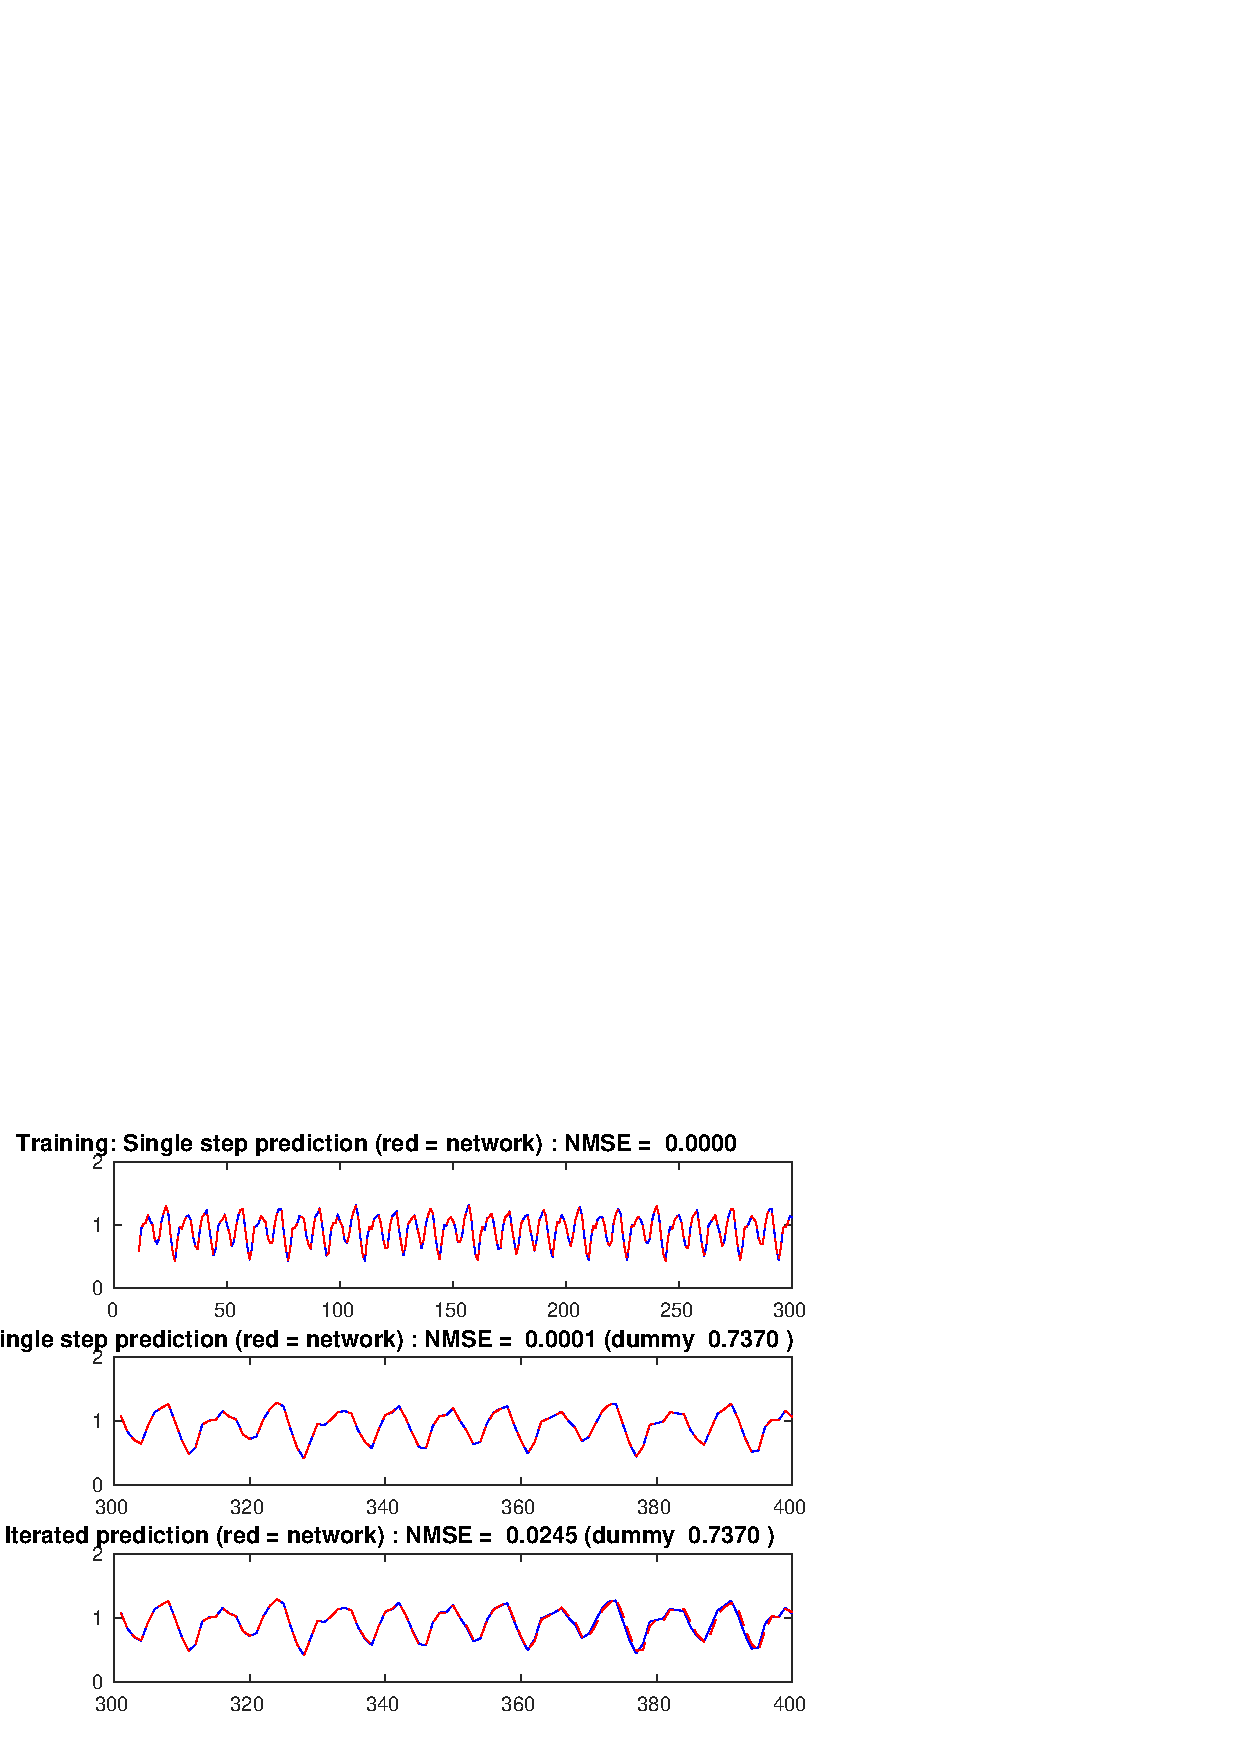
\includegraphics[scale=.8]{12_21_nodes_levenberg}
         \caption{Performance for single-layer network with 21 hidden nodes and
         the LM algorithm on the Mackey-Glass data.}
         \label{fig:12}
      \end{figure}
      
      For the Mackey-Glass data set, the output proved to be significantly
      easier to predict than in previous cases. Naturally, this ought to be
      because of the underlying function here being definite, which results in
      the fact that the training set is not only periodically the same, but also
      identical to the test data set. It is thereby of no great surprise that
      the error achieved is as small as it happens to be. The architecture does
      furthermore not seem to play a significant role in this case, as many
      investigated nets proved to be equally able to predict the test data. 

   \subsection{Challenge Exercise}
      With respect only to the ability to minimize the fraction of missed
      classifications, a 4-fold cross validation was implemented. Uses of
      a larger amount of folds rendered results not as good as the 4-fold, which
      ought to be because of the slim size of the data set (only 384 data points
      in total, rendering a validation set of 96 points in a 4-fold
      cross-validation). It is
      however questionable which measure of performance should be used in
      evaluating the networks; in
      principle, the area under the ROC curve can be calculated, although it
      proved practically a hard feat to do so. In general however, it would 
      seem as if the back-propagating learning algorithms provide better
      networks on average. 

      Out of all the algorithms and networks simulated, the best was the 8-node
      network utilizing the Resilient Backpropagation method, with a correct
      match performance of 76.3 \%. (Data included in attached file output.dat.)

      Finally, when evaluating the correlation between the different input
      factors and the targets in the training set given, one can see that almost
      all dimensions seem to have very small direct effect on the target result,
      aside from one single factor (which like all the others is unknown), that
      instead has a clear linear trend relative to the target data. This however
      requires contextual consideration, as several of the non-correlated
      factors might have a combined effect on the outcome. Nontheless, the
      direct correlation between the single factor mentioned ought to be of
      importance.

   \section{Concluding remarks}
     It is fascinating to see how a fairly simple neural network can perform so
     well at many complex tasks. Nevertheless, the results here shows that it is
     perhaps more than anything important to evaluate an ensemble of networks in
     order to be able to draw conclusions about an architecture's or algorithm's
     performance. 

     Although many of the more advanced learning algorithms were significantly
     slower from a computational perspective, the ability of many of them to
     predict as well time series as functions provided a large incentive to
     indeed use them for many of the tasks.  

     In summary, the capabilites of neural nets are nothing less than
     extraordinary -- especially in the way that such a vast variety of 
     different problems can be solved by so similar structures and architectures. 

   \begin{thebibliography}{99}
   \bibitem{lecnotes}
     Mattias Ohlsson,
     \emph{Lecture notes, Artificial Neural Networks},
     Department of Astronomy and Theoretical Physics,
     Lund University,
     2015.
   \bibitem{excnotes}
     Mattias Ohlsson,
     \emph{Exercise 1: Perceptrons and Multi-layer perceptrons for
     classification and prediction of time series},
     Department of Astronomy and Theoretical Physics,
     Lund University,
     2015.
\end{thebibliography}
%\newpage
%\appendix
%\section{Code}
 %  \label{sec:code}
 %  \lstinputlisting[language=Java]{Common.java}
 %  \lstinputlisting[language=Java]{Forest.java}
 %  \lstinputlisting[language=Java]{Square.java}
 %  \lstinputlisting[language=Java]{Food.java}
 %  \lstinputlisting[language=Java]{Anthill.java}
 %  \lstinputlisting[language=Java]{AntPanel.java}
 %  \lstinputlisting[language=Java]{Ant.java}
 %  \lstinputlisting[language=Java]{SpeedAnt.java}
 %  \lstinputlisting[language=Java]{BruteAnt.java}
\end{document}

